
\documentclass[]{report}

\usepackage{subfig}
\usepackage{tikz}
\usepackage{pgfplots}
\usepackage{pgfplotstable}
\usepackage{booktabs}
\usepackage{hyperref}

% Title Page
\title{What I did at Fraunhofer IGD}
\author{Seyedmorteza Mostajabodaveh}


\begin{document}
%\maketitle

%\begin{abstract}
%In November 2014, I moved to Darmstadt to work in Fraunhofer IGD and do my master thesis. In this report, I will present the tasks which I have done beside my master thesis at Fraunhofer IGD as Hiwi. Additionally, my supervisor Andreas Dietrich (\href{andi.dietrich@googlemail.com}{andi.dietrich@googlemail.com}) which was working at Fraunhofer IGD before was directing me toward these tasks. You can contact him for more information.
%\end{abstract}

\begin{figure}[!ht]
	\subfloat{%
		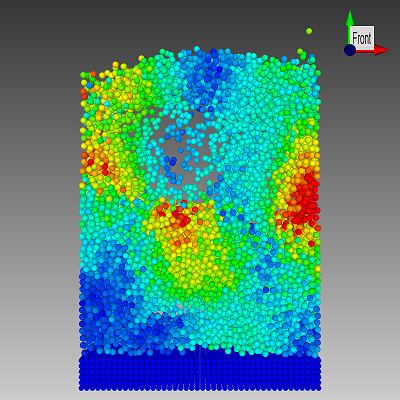
\includegraphics[width=0.2\textwidth]{./figs/particles/new/1.png}
	}
	\hfill
	\subfloat{%
		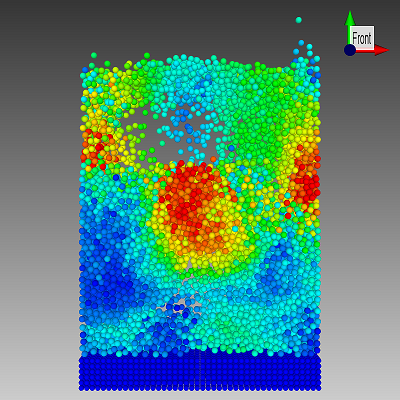
\includegraphics[width=0.2\textwidth]{./figs/particles/new/2.png}
	}
	\hfill
	\subfloat{%
		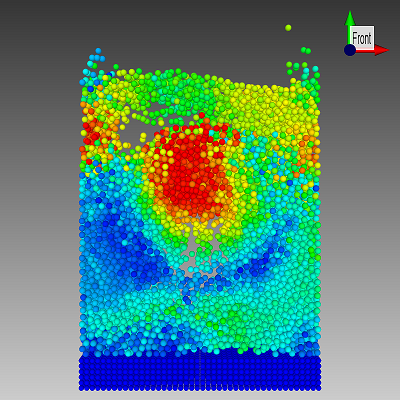
\includegraphics[width=0.2\textwidth]{./figs/particles/new/3.png}
	}
	\hfill
	\subfloat{%
		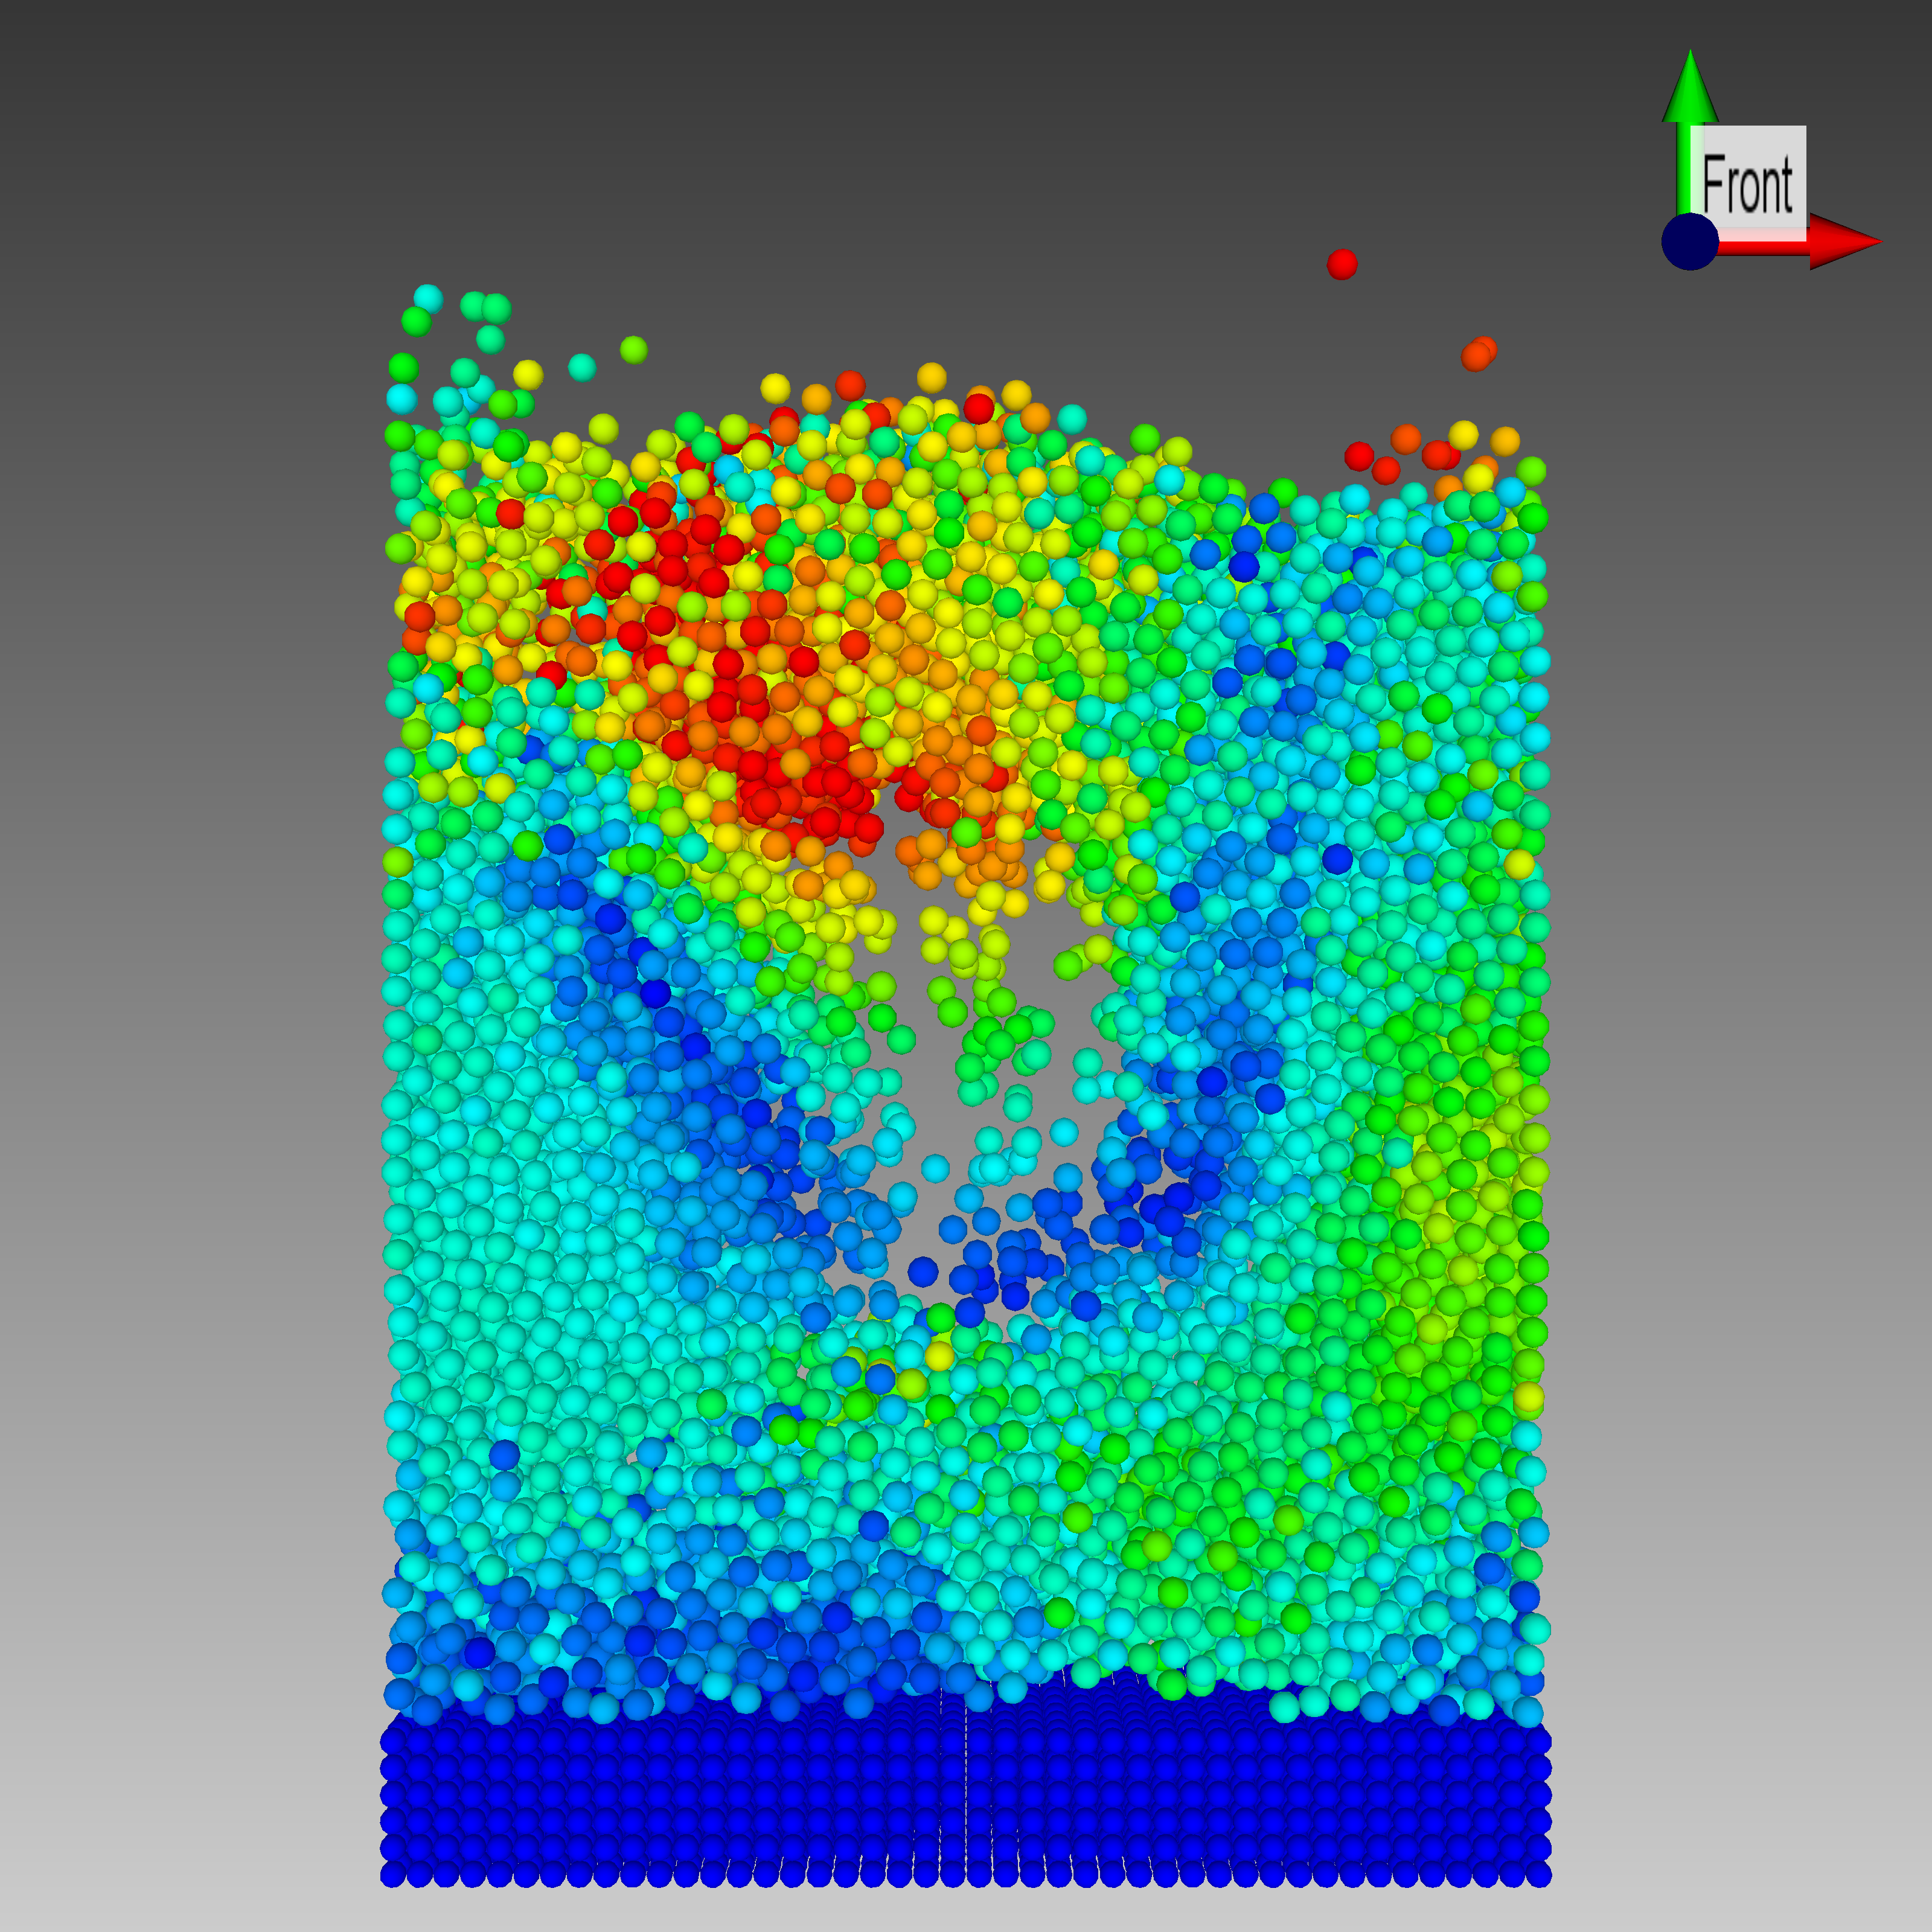
\includegraphics[width=0.2\textwidth]{./figs/particles/new/4.png}
	}
	\hfill
	\subfloat{%
		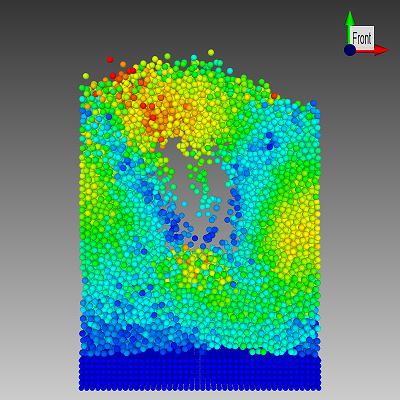
\includegraphics[width=0.2\textwidth]{./figs/particles/new/5.png}
	}
	\hfill
	\subfloat{%
		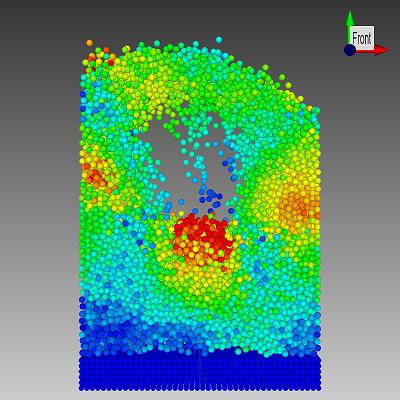
\includegraphics[width=0.2\textwidth]{./figs/particles/new/6.png}
	}
	\hfill
	\subfloat{%
		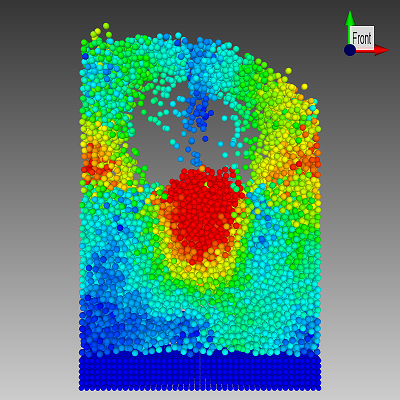
\includegraphics[width=0.2\textwidth]{./figs/particles/new/7.png}
	}
	\hfill
	\subfloat{%
		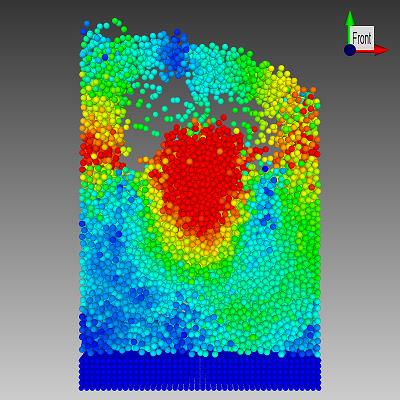
\includegraphics[width=0.2\textwidth]{./figs/particles/new/8.png}
	}
	\hfill
	\subfloat{%
		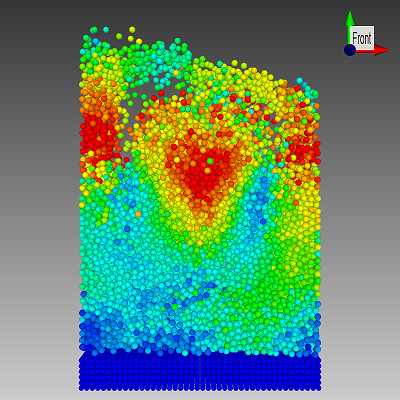
\includegraphics[width=0.2\textwidth]{./figs/particles/new/9.png}
	}
	\hfill
	\subfloat{%
		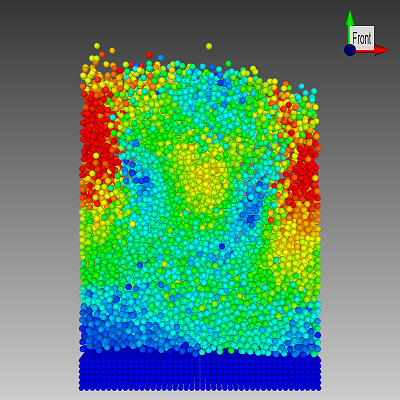
\includegraphics[width=0.2\textwidth]{./figs/particles/new/10.png}
	}
	\hfill
	\subfloat{%
		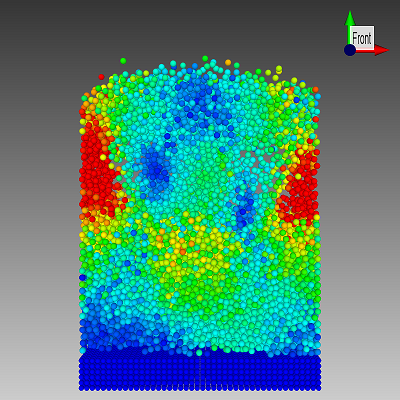
\includegraphics[width=0.2\textwidth]{./figs/particles/new/11.png}
	}
	\hfill
	\subfloat{%
		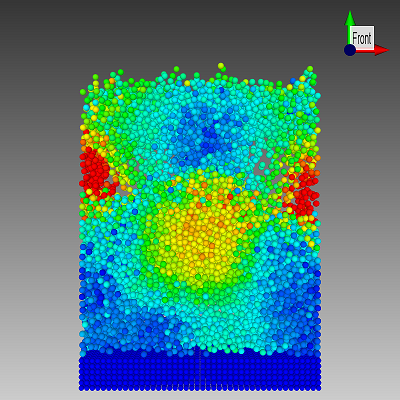
\includegraphics[width=0.2\textwidth]{./figs/particles/new/12.png}
	}
	\hfill
	\caption[Query particles from HBase database and their visualization]{\textbf{Particles in different timesteps} are queried from HBase database. The velocity vectors for all particles are queried separately. The particles are color-mapped based on their velocity magnitude.}
	\label{fig:particles}
\end{figure}

\begin{figure}[!ht]
	\subfloat{%
		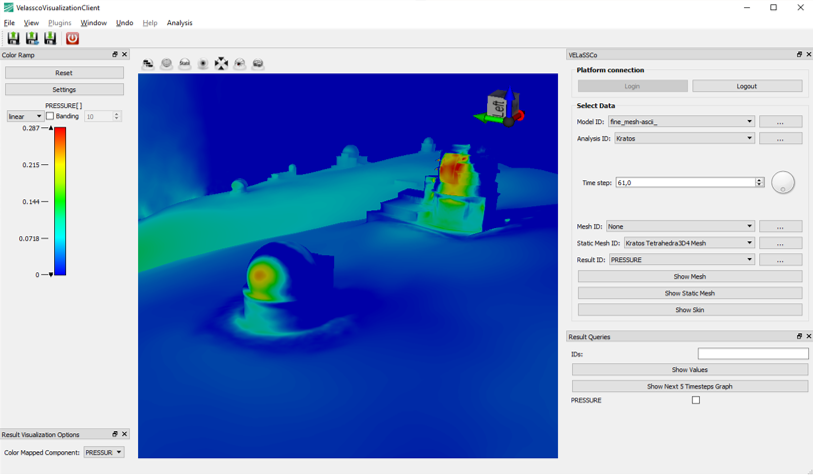
\includegraphics[width=0.53\textwidth]{./figs/velassco/telescope1.png}
	}
	\hfill
	\subfloat{%
		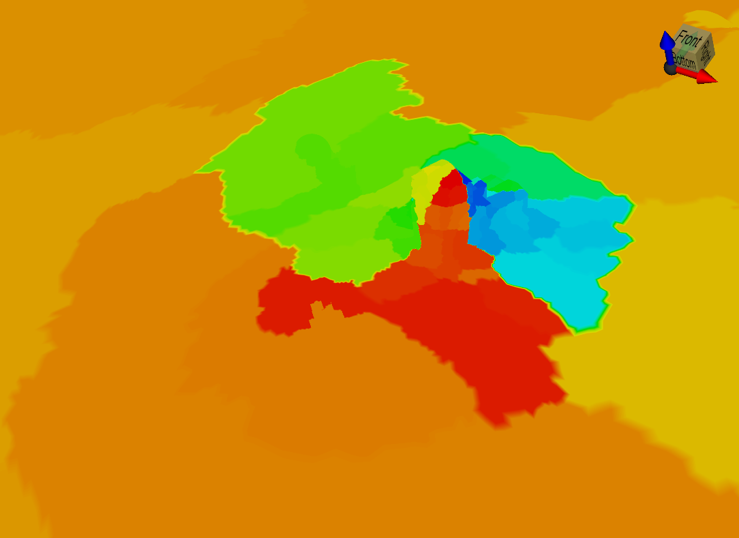
\includegraphics[width=0.43\textwidth]{./figs/velassco/telescope2.png}
	}
	\hfill
	\caption[Telescope Boundary Mesh]{\textbf{Telescope simulation boundary mesh} with color-mapped pressure values in left figure and partition IDs in right figure. First the telescope boundary mesh computation is queried from the HBase database. It computes the boundaries of the mesh and the result mesh is sent back to the client. The client query specific results on the boundary mesh vertices. The colormapping is done on the clinet side.}
	\label{fig:telescope}
\end{figure}

\begin{figure}[!ht]
	\subfloat{%
		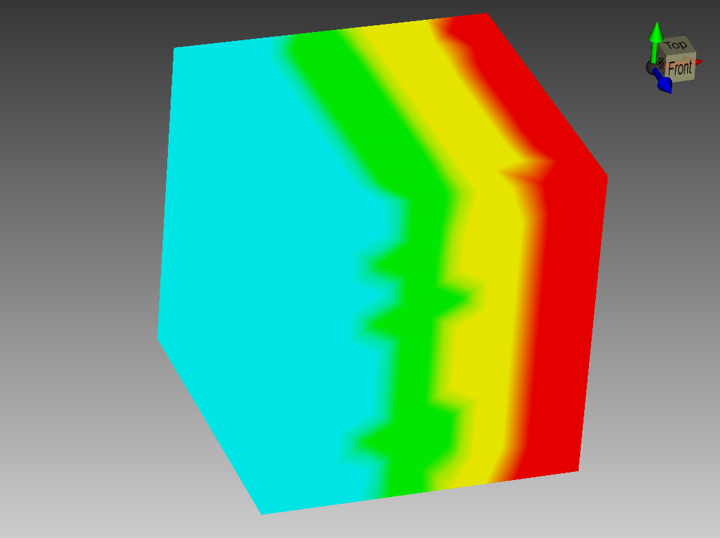
\includegraphics[width=0.375\textwidth]{./figs/velassco/getmesh1.png}
	}
	\hfill
	\subfloat{%
		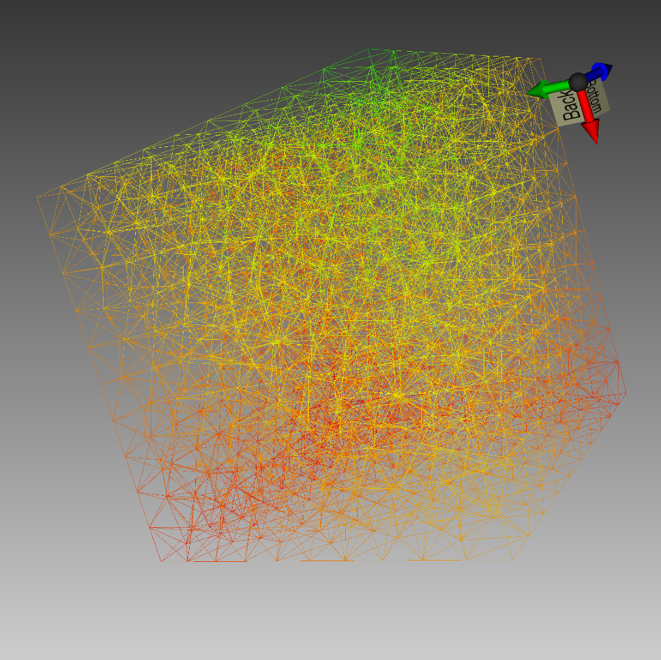
\includegraphics[width=0.28\textwidth]{./figs/velassco/getmesh2.png}
	}
	\hfill
	\subfloat{%
		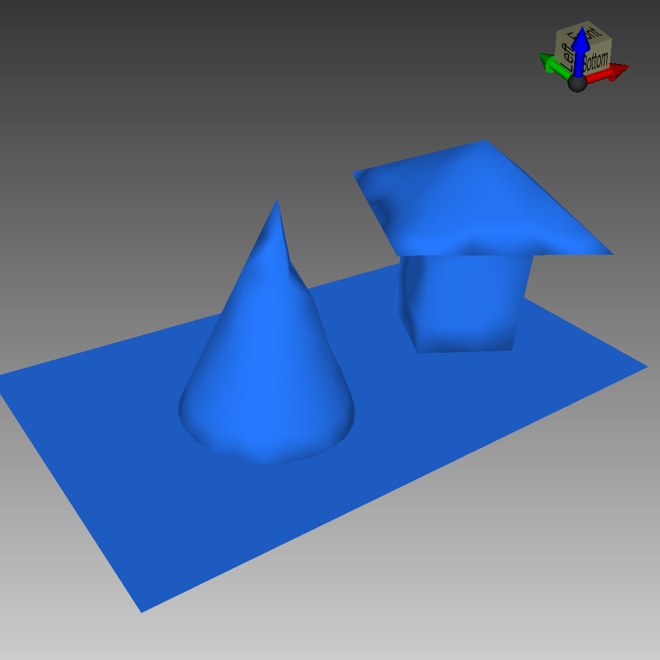
\includegraphics[width=0.28\textwidth]{./figs/velassco/getmesh3.png}
	}
	\hfill
	\caption[Getting simulation mesh informaton]{\textbf{Querying simulation mesh} from HBase database. The results on the simulation mesh vertices are queried separaretly and visualized using colormapping.}
	\label{fig:sim_meshes}
\end{figure}


\textbf{VELaSSCo project}. "Visualization for Extremely Large Scale Scientific Computing" known as VELaSSCo is an EC funded project which deals with end-user visualization of big data. The idea behind this project is to store the datasets on a distributed database like HBase (Hadoop) or EDM. The user can query a specific part of data in the database or a specific operation on the data in the database. The user's query is processed on the HPC and the result is sent back in a GPU-friendly format for the client to be visualized e.g.~Figure \ref{fig:telescope} shows the boundary mesh of telescope dataset which the pressure values on its surface are color-mapped. First, the client queries for the mesh boundary. The HPC computes the boundary of the mesh and sends it back to the client. The client sends another query to request for pressure values of the vertices on the boundary mesh. It uses received data to visualize the boundary with pressure values color-mapped on its surface. Figure \ref{fig:particles} shows the particles in different timesteps which their velocity magnitude is color-mapped. The client queries the particle's position and radius in each timestep. The velocity vectors for the particles are queried afterwards. The velocity magnitude is computed on the client side, and used to color-map the particles' visualization. 

In this project, I mainly focused on implementing two direct result queries on the HPC side. They are used to return the result values on a list of vertex indices, and mesh drawing data. Mesh drawing data query result requires to be returned in a GPU friendly format. Therefore, it can be copied directly directly into OpenGL buffers to draw. I implemented these two queries using Thrift C++ API. On the client side, I implemented a plug-in to support VELaSSCo Plugin for indoor application called Rapid Prototyping Environment (RPE). This plugin supports:
  
\begin{itemize}
	\item query for available model information, their analysis, results, meshes, and static meshes.
	\item Query for computing boundary mesh of a specific dataset (Figure \ref{fig:telescope}).
	\item Query for computing discrete-to-continuum surface for DEM cases.
	\item Query for Finite Element Meshes (FEM) / Discrete Element Meshes (DEM) and render them (Figure \ref{fig:sim_meshes}).
	\item Query for results on a specific node in a specific timestep or a vertex's results evaluation in all time steps.
	\item Query for particles in different timesteps for DEM cases and create an animation which can be play-backed.
\end{itemize}

\begin{figure}[!ht]
	\centering
	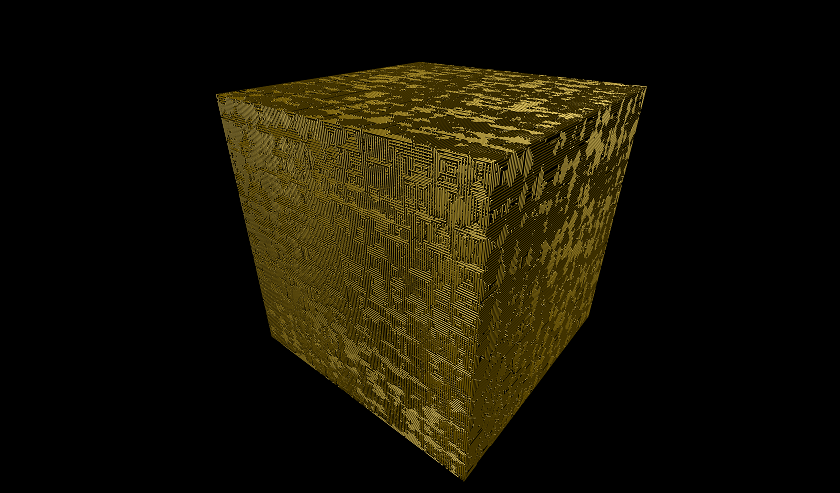
\includegraphics[width=0.90\textwidth]{./figs/pipecube.png}
	\caption[Pipecube]{\textbf{Pipecube} made of more than 15.6 million pipes, ray-traced on a 1920x1200 display on 17 fps using Intel Embree on an Intel Core i7-4960X.}
	\label{fig:pipecube}
\end{figure}

\begin{figure}[!ht]
	\subfloat{%
		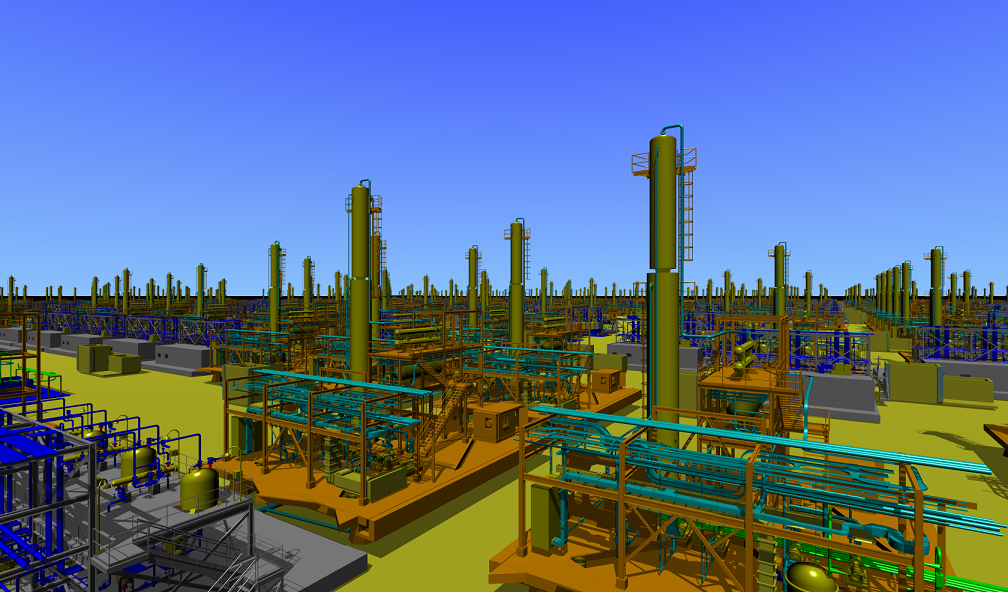
\includegraphics[width=0.3\textwidth]{./figs/embree1.png}
	}
	\hfill
	\subfloat{%
		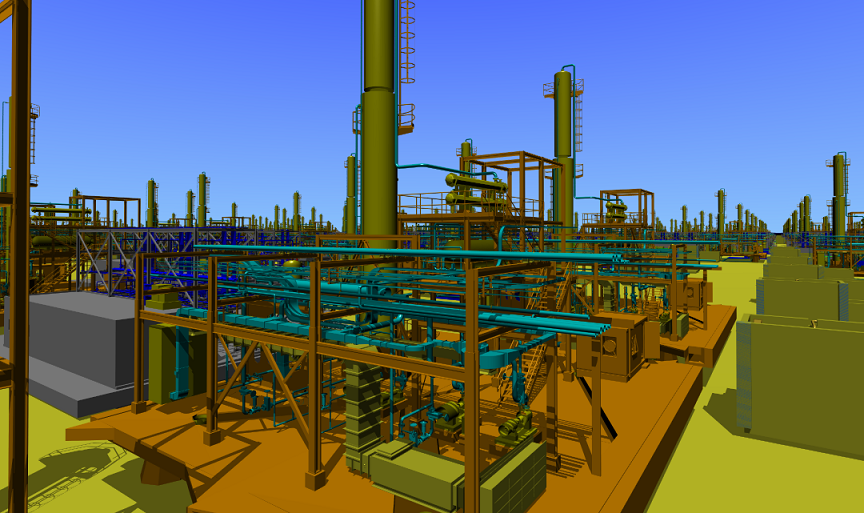
\includegraphics[width=0.3\textwidth]{./figs/embree2.png}
	}
	\hfill
	\subfloat{%
		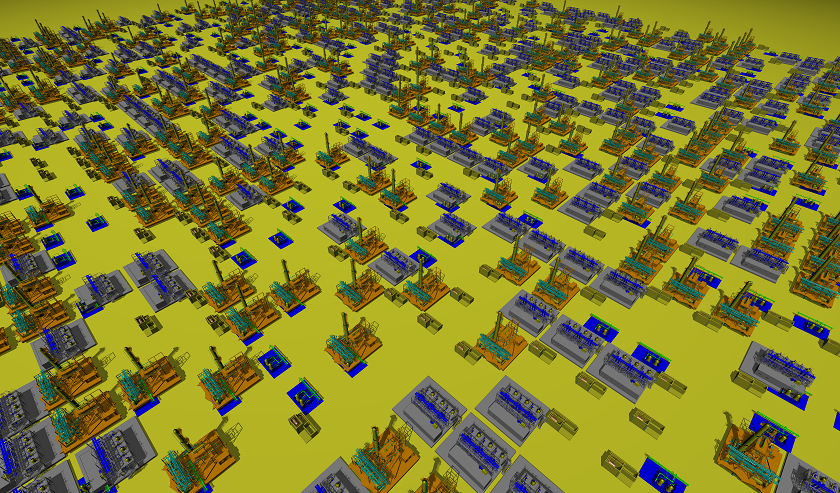
\includegraphics[width=0.3\textwidth]{./figs/embree3.png}
	}
	\hfill
	\caption[Factory ray-tracing]{\textbf{Factory ray-tracing with Embree}.}
	\label{fig:embreeFactory}
\end{figure}

\begin{figure}[!ht]
	\subfloat{%
		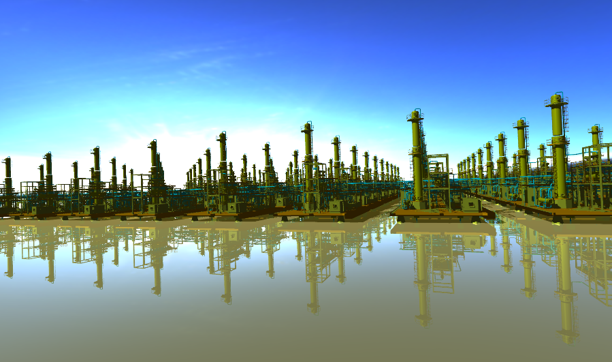
\includegraphics[width=0.3\textwidth]{./figs/optix1.png}
	}
	\hfill
	\subfloat{%
		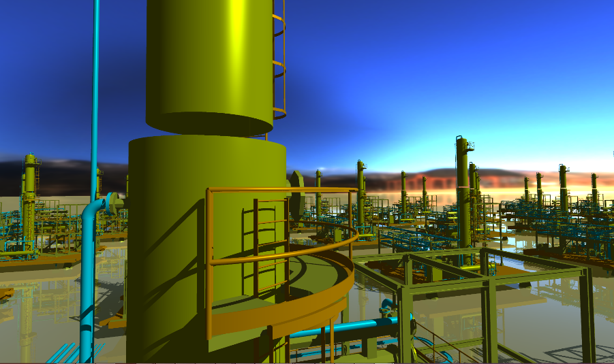
\includegraphics[width=0.3\textwidth]{./figs/optix2.png}
	}
	\hfill
	\subfloat{%
		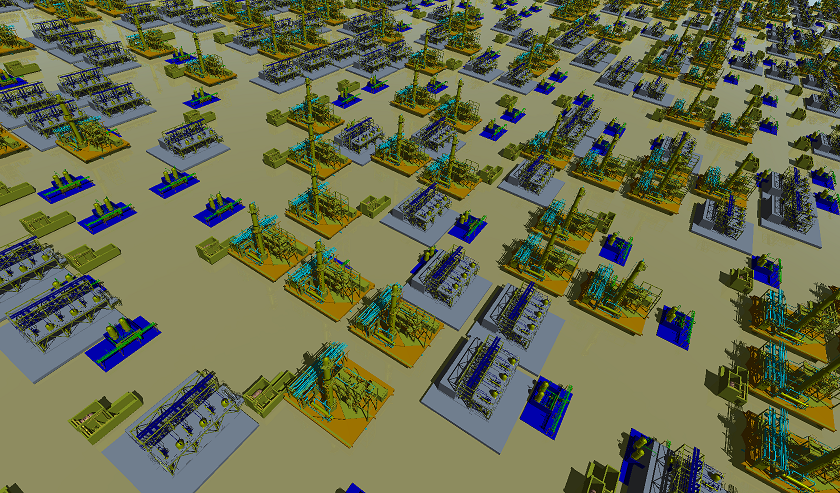
\includegraphics[width=0.3\textwidth]{./figs/optix3.png}
	}
	\hfill
	\caption[Factory ray-tracing]{\textbf{Factory ray-tracing with Optix}.}
	\label{fig:optixFactory}
\end{figure}

\begin{figure}[!ht]
	\centering
	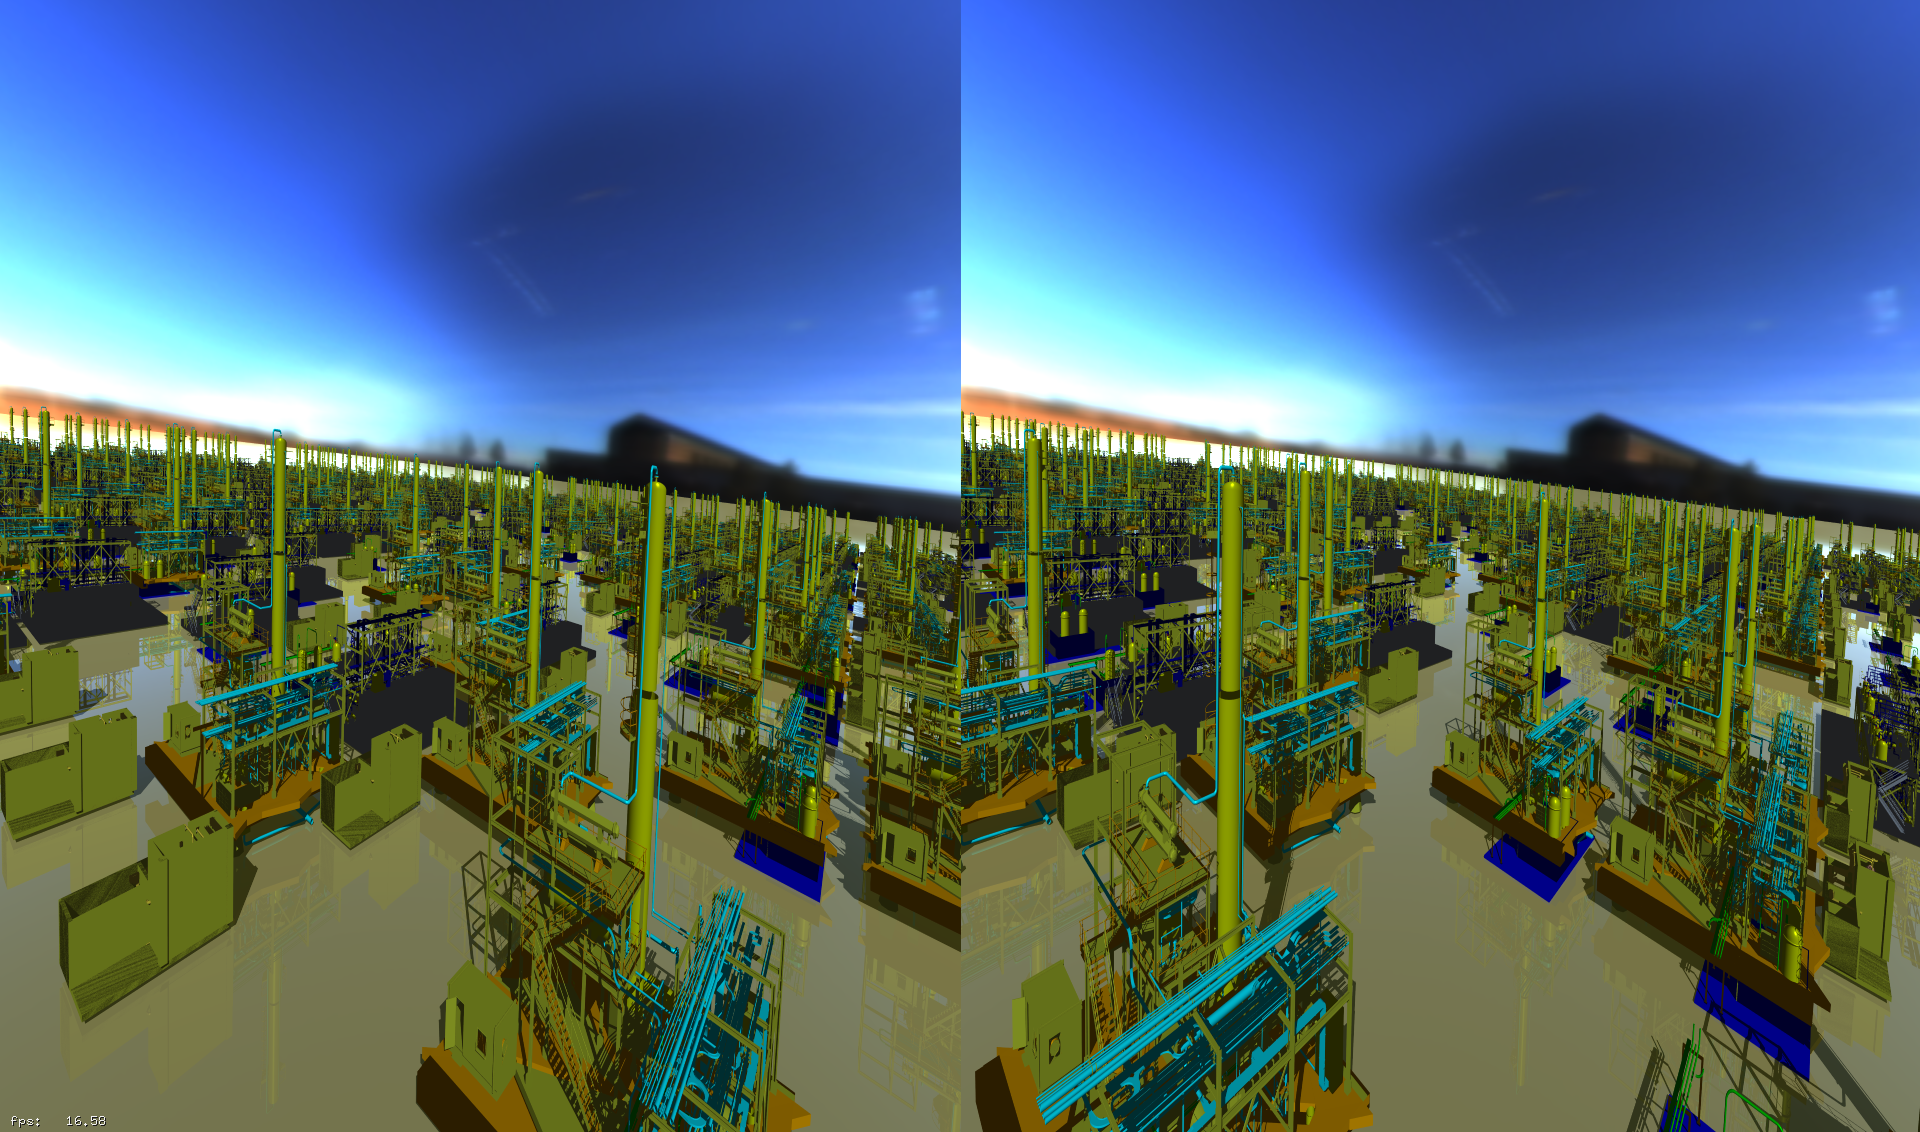
\includegraphics[width=0.90\textwidth]{./figs/stereo.png}
	\caption[Factory ray-tracing (Stereoscopic view)]{\textbf{Factory ray-tracing (Stereoscopic view)}.}
	\label{fig:stereoFactory}
\end{figure}

\textbf{Ray-tracing higher-order primitives}. This task starts with a simple example which was rendering of a pipecube using pipes which are made of two spheres and one cylinder. To speed up renderer, and to get a smooth final image instead of triangulating the primitives, the ray-primitive intersection is computed analytically. The GPU version was implemented by Andreas Dietrich using NVIDIA Optix and I implemented the CPU version using Intel Embree. The CPU version was able to handle very big and smooth pipecubes (Figure \ref{fig:pipecube}). This was an starting idea for implementing a version which uses the AVEVA's RVM files to produce the factory models with higher order primitives (Sphere, Box, ...) and then ray-trace it on CPU or GPU. I implemented a factory viewer in two version (NVIDIA Optix and Intel Embree one) which ray-traces a group of factories(figure\ref{fig:embreeFactory} shows the output image achieved by utilizing Intel Embree on Intel Core i7 CPU. Figure \ref{fig:optixFactory} shows the NVIDIA Optix output image on a NVIDIA Geforce GTX 980). Additionally, the GPU version was supporting 3D stereoscopic output for 3D projectors (figure \ref{fig:stereoFactory}).

\begin{figure}[!ht]
	\centering
	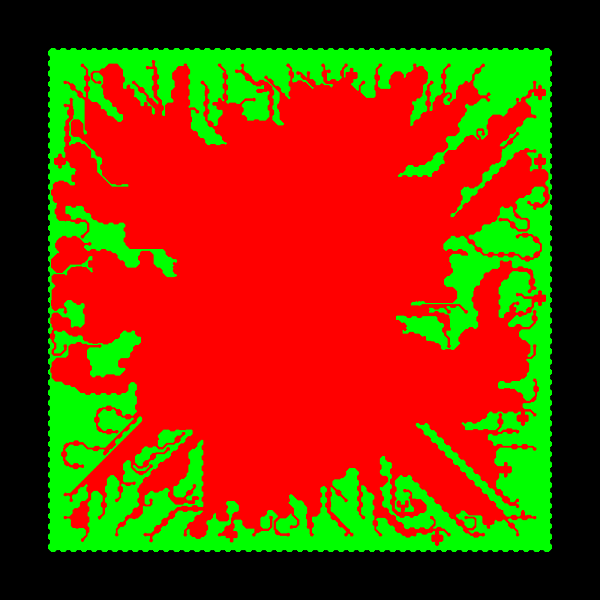
\includegraphics[width=0.90\textwidth]{./figs/rasterizer2D.png}
	\caption[PCB 2D Rasterization]{\textbf{Software PCB rasterization} done 107 fps on Core i7-4960X.}
	\label{fig:twodimRaster}
\end{figure}

\textbf{PCB board software rasterizer}. Implementing a software rasterizer which determines if a pixel on the screen is in the PCB board, which is going to be printed, or it is part of holes. The application gets a group of positive and negative polygons as input. Figure \ref{fig:twodimRaster} shows the output of the application for sample case. For each pixel, a counter is assumed which is initialized to zero. For each polygon, the pixel is examined. If the pixel is inside a negative polygon the counter is decremented, if it is inside a positive polygon the counter is incremented. Finally, pixels with positive counter value are inside the PCB board (shown as green), pixels with negative values are inside the holes (shown as red) which means the board should be cut to achieve them, and pixels which the counter's value is zero are not in the PCB board area (can be encountered as hole). To speed up point-inside-polygon process, a grid acceleration structure is used which its elements store the polygon references that overlap them. The point-inside-polygon check is done only for polygons which their references is stored in the grid's element which the pixel resides in.

\begin{figure}[!ht]
	\subfloat[Airport Scene\label{subfig-1:VR}]{%
		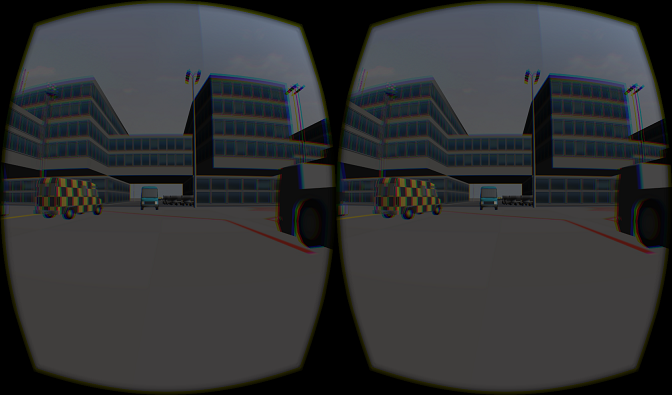
\includegraphics[width=0.48\textwidth]{./figs/Vr1.png}
	}
	\hfill
	\subfloat[Forklift Driving\label{subfig-2:VR}]{%
		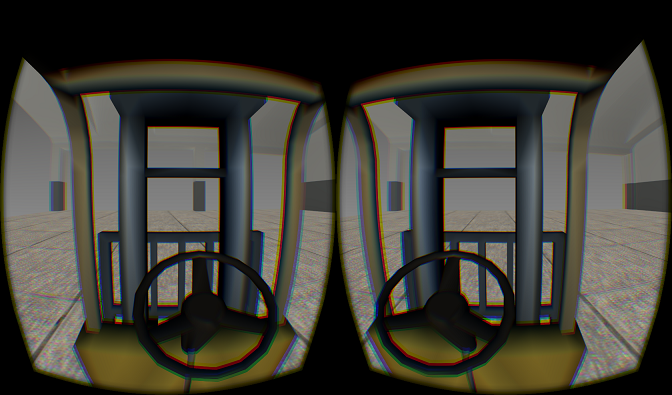
\includegraphics[width=0.48\textwidth]{./figs/Vr2.png}
	}
	\caption[Virtual Reality]{\textbf{Virtual Reality} Projects.}
	\label{fig:VR}
\end{figure}

\textbf{Virtual Reality}. I fixed some bugs in Oculus Rift plug-in of indoor visualization software called Rapid Prototyping Environment (RPE). Additionally, I extended the plug-in for specific projects, to support a player camera inside the scene. The user was able to move through the scene. Furthermore, I extended the plug-in to add leap motion support. The user is able to control the camera with specific gestures (rotating with swiping hand, zooming in/out by points hand inside/outside). Figure \ref{fig:VR} shows two screenshots of the VR projects that I did at Fraunhofer IGD. 

\begin{figure}[!ht]
	\centering
	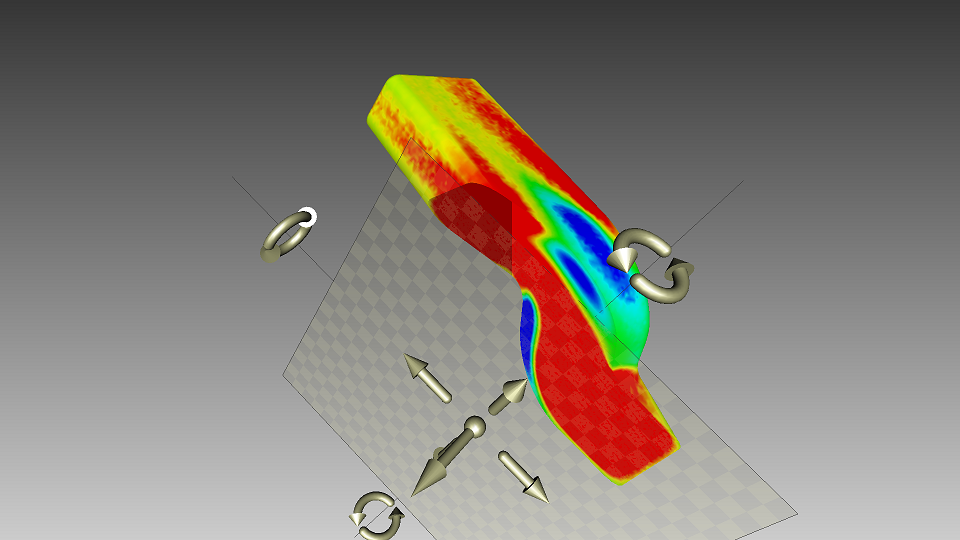
\includegraphics[width=0.90\textwidth]{./figs/crosssection.png}
	\caption[Cross section]{\textbf{Cross section} of wind tunnel dataset.}
	\label{fig:crossection}
\end{figure}


\begin{figure}[!ht]
	\centering
	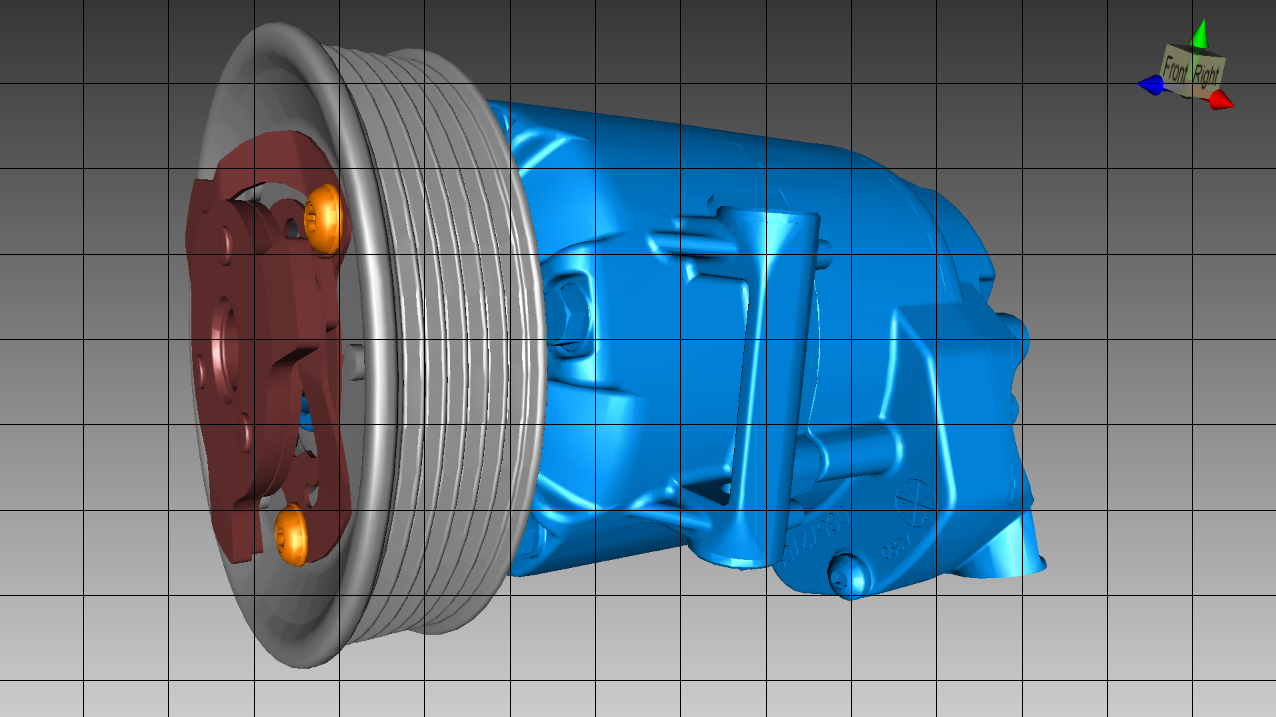
\includegraphics[width=0.90\textwidth]{./figs/highresscreenshot.png}
	\caption[Extremely high resolution screenshot capturing]{\textbf{Extremely high resolution screenshot capturing}.}
	\label{fig:highres}
\end{figure}

\begin{figure}[!ht]
	\centering
	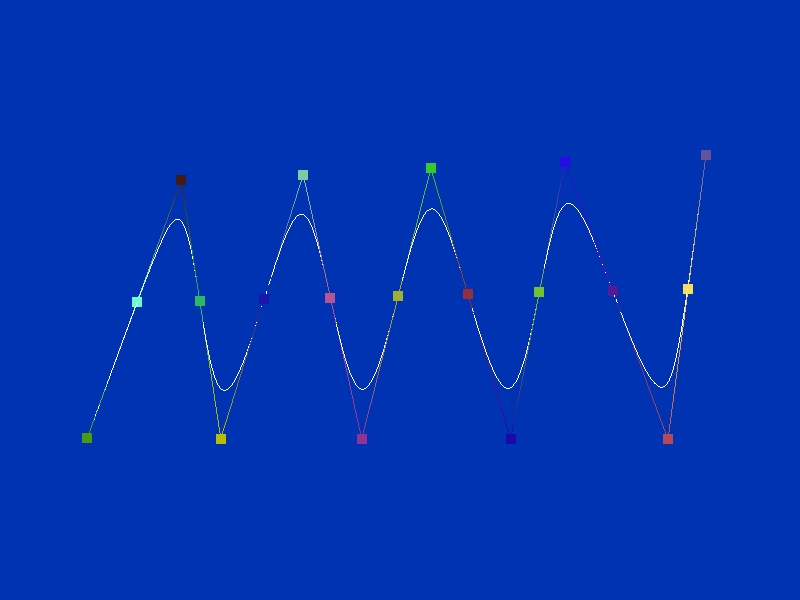
\includegraphics[width=0.90\textwidth]{./figs/bspline.png}
	\caption[B-Spline GPU Tessellation]{\textbf{Evaluating B-Spline on GPU} using a tessellation shader.}
	\label{fig:bspline}
\end{figure}

\begin{figure}[!ht]
	\centering
	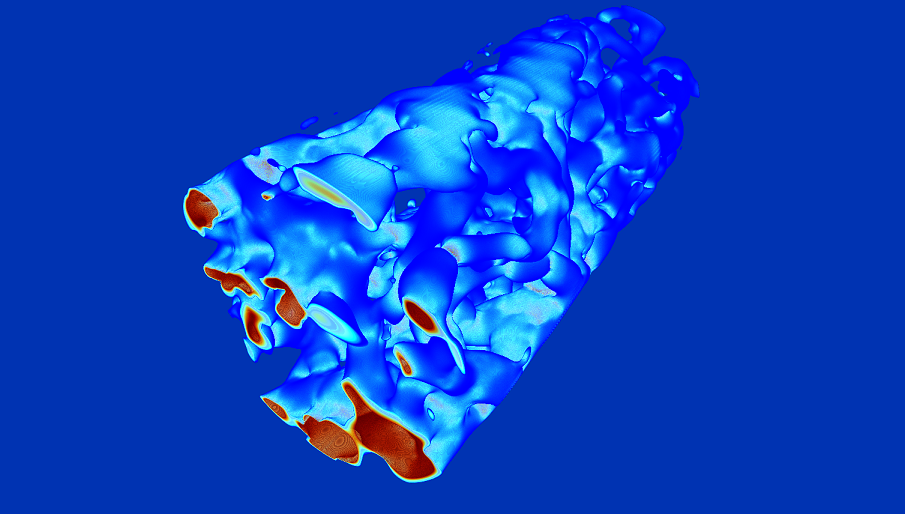
\includegraphics[width=0.90\textwidth]{./figs/dvr.png}
	\caption[Direct volume rendering]{\textbf{Direct volume rendering} of ground water flow dataset's simulation from Florida International University. Colors represent the water's velocity at each point.}
	\label{fig:dvr}
\end{figure}

\hfill

\textbf{Other Tasks}:
\begin{itemize}
	\item Implementing cross-section algorithm for unstructured simulation mesh types (Figure \ref{fig:crossection}).
	\item Adding very large screenshot capturing feature to RPE (Figure \ref{fig:highres}).
	\item Evaluating B-Spline on the GPU using tessellation shader (Figure \ref{fig:bspline}).
	\item Direct volume rendering by implementing a ray marching fragment shader (Figure \ref{fig:dvr}).
\end{itemize}

\begin{figure}[!ht]
	\subfloat[\label{IDP_overview:fig1}]{%
		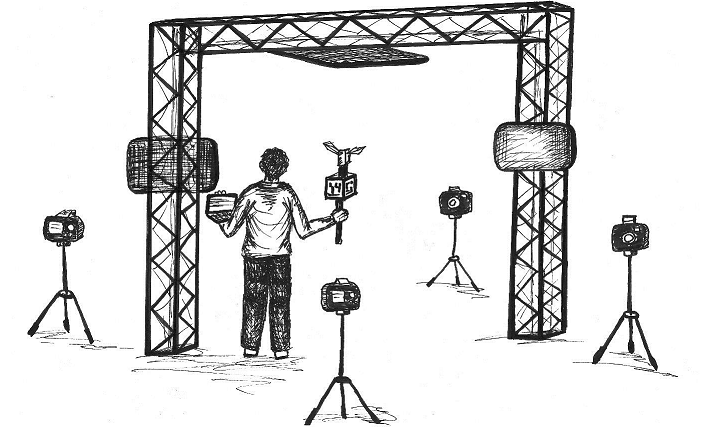
\includegraphics[width=0.58\textwidth]{./figs/idp_overview.png}
	}
	\hfill
	\subfloat[\label{IDP_overview:fig2}]{%
		\includegraphics[width=0.38\textwidth]{./figs/idp_userAssist.png}
	}
	\hfill
	\caption[Factory ray-tracing]{\textbf{3D-Visualization of electromagnetic field strength distribution} overview. The right figure shows how the application assists the user to collect enough data during measurement. For each regular grid's element a bar will appear which its height and color show how much data is collected for that part of the environment. The bars are rendered in transparent to let the user see through them.}
	\label{fig:IDP_overview}
\end{figure}

\begin{figure}[!ht]
	\subfloat{%
		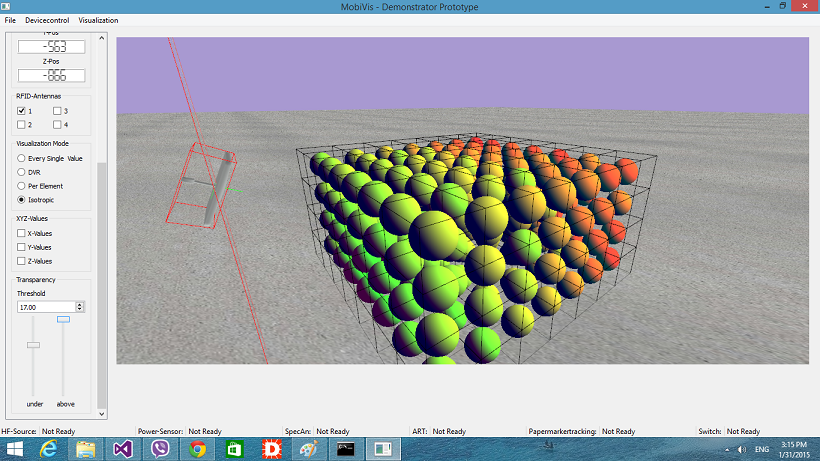
\includegraphics[width=0.3\textwidth]{./figs/idp1.png}
	}
	\hfill
	\subfloat{%
		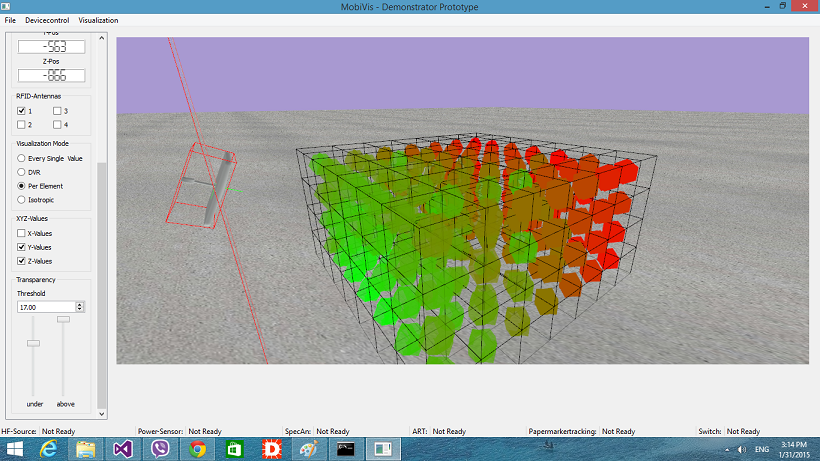
\includegraphics[width=0.3\textwidth]{./figs/idp2.png}
	}
	\hfill
	\subfloat{%
		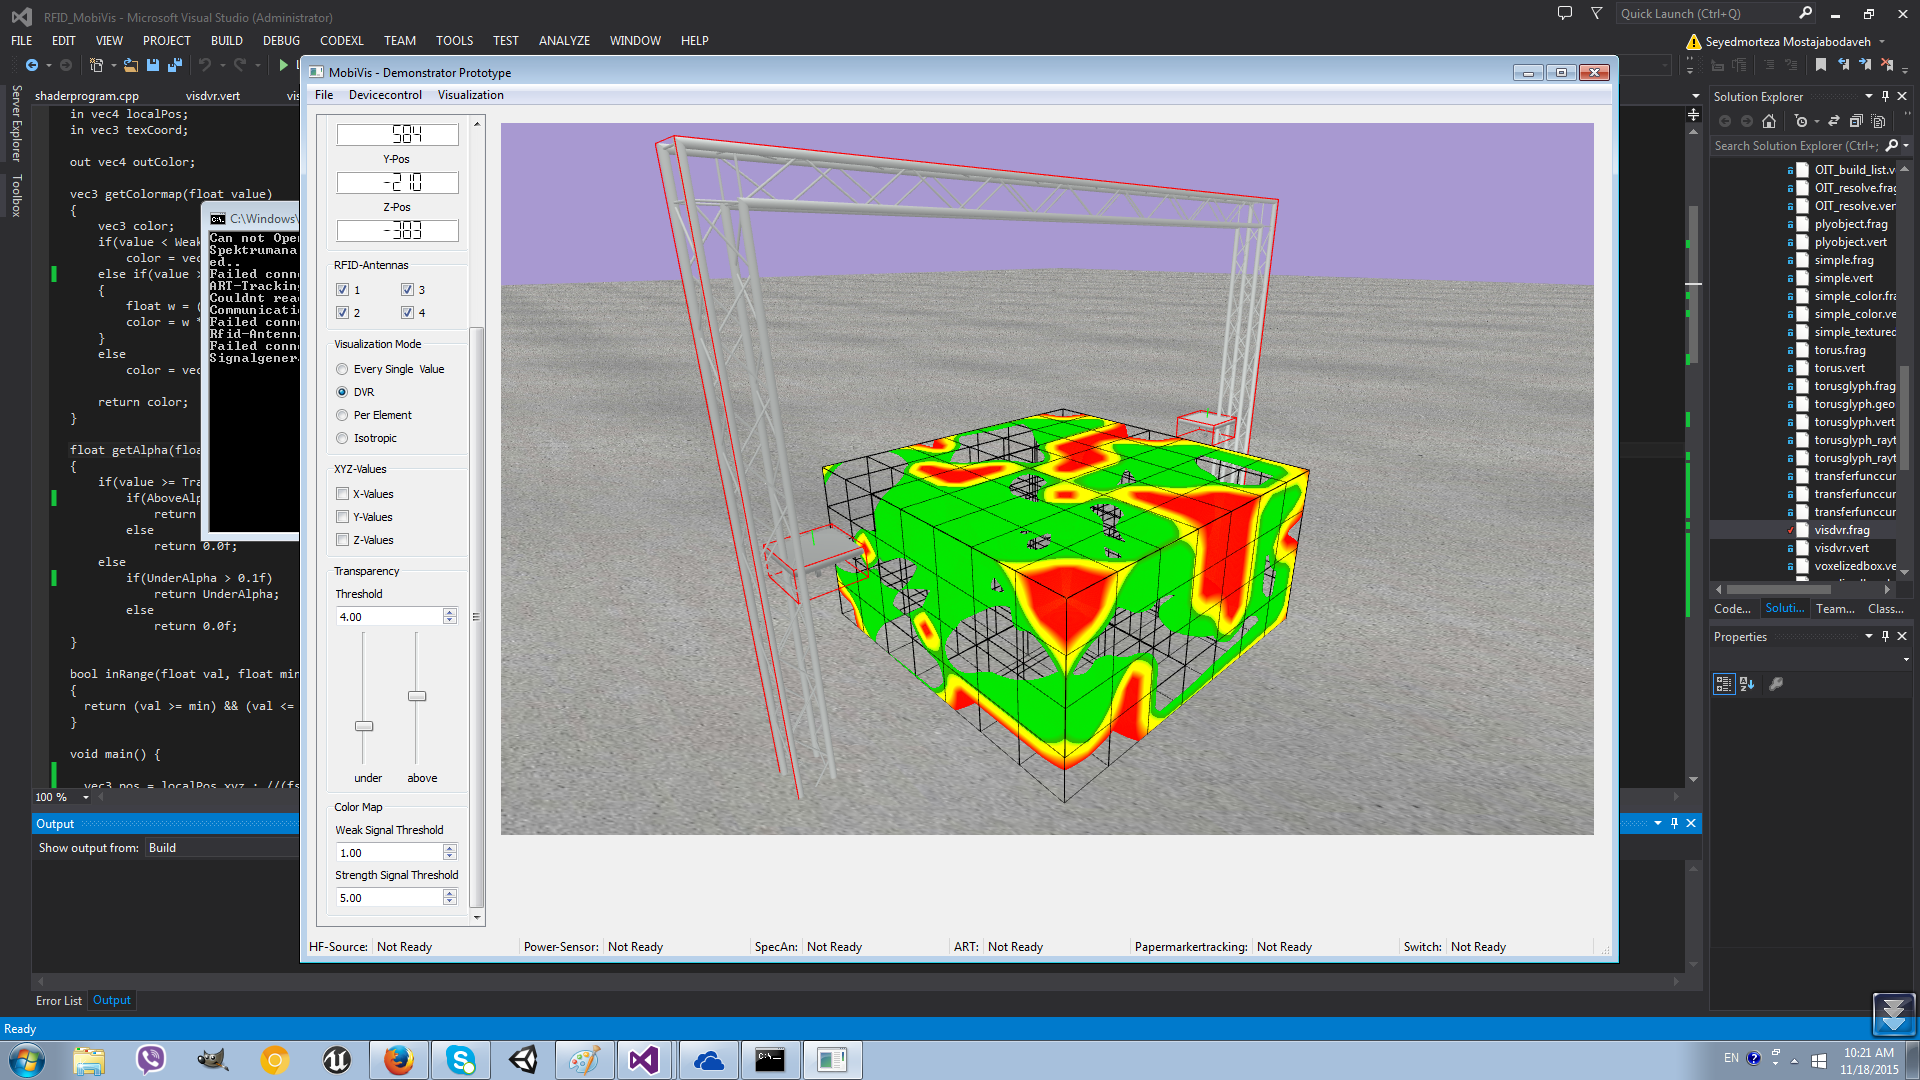
\includegraphics[width=0.3\textwidth]{./figs/idp3.png}
	}
	\hfill
	\caption[Factory ray-tracing]{\textbf{Magnetic field} visualization using different techniques.}
	\label{fig:IDP_results}
\end{figure}
 
 \textbf{Interdisciplinary Project (IDP): 3D-Visualization of electromagnetic field strength distribution}. To activate and detect the passive RFIDs which are passed through a RFID detection gate correctly, a specific range of magnetic field in an area around the gate is expected. The goal of the project is to assist the user to measure magnetic field in a specific area around the gate and visualize the values to detect the areas around the gate that has high/low magnetic field strength. To measure the magnetic field in a specific point, a measurement antenna is used. To keep track of the antenna's position, it is equipped with retro-reflective markers. The gate is surrounded with four ART-trackers which track the marker positions (Figure \ref{IDP_overview:fig1}). The user is able to work with the system through a remote controller. Using a separate marker, the user defines the gate dimension and position, antenna positions to initialize the 3D world. The user uses the same marker to define the area of interest for measurement to the application. During the measurement, application helps the user to collect enough data to make the measurements accurate (Figure \ref{IDP_overview:fig2}). When the data is collected, the user is able to visualize the collected data in each direction, and its magnitude using sphere or torus glyphs. Additionally, the collected values can be displayed more clearly by rendering the collected volume of data. Figure \ref{fig:IDP_results} shows some of the achieved results.

\textbf{Homepage}. My homepage page can found here:

\url{https://www.mmostajab.com}
 
\textbf{GitHub Page}. My GitHub page can found here:
 
\url{https://github.com/mmostajab}

Some of my main projects are private and cannot be viewed here. It will be my pleasure to add you as contributor to have a look on them, also.  
  
 
 \textbf{Older Projects} can be found here:
 
 \url{https://mmostajab.com/old-projects/}
 
 
\end{document}          
